\vspace{2em}
\subsection{Ερώτημα 3-1-4}
Εν συνεχεία τα προηγούμενα πειράματα εκτελέστηκαν σε πραγματικό σύστημα 4
physical cores με τεχνολογία hyperthreading, συνεπώς με 8 logical cores. Ο
αριθμός επαναλήψεων τέθηκε ίσος με 150000000. Ακολουθούν τα διαγράμματα του χρόνου:

\begin{minipage}{\textwidth}
   \begin{center}
      \fbox{\textlatin{\textbf{\textit{Grain Size: 1}}}}\\
      \vspace{3mm}
      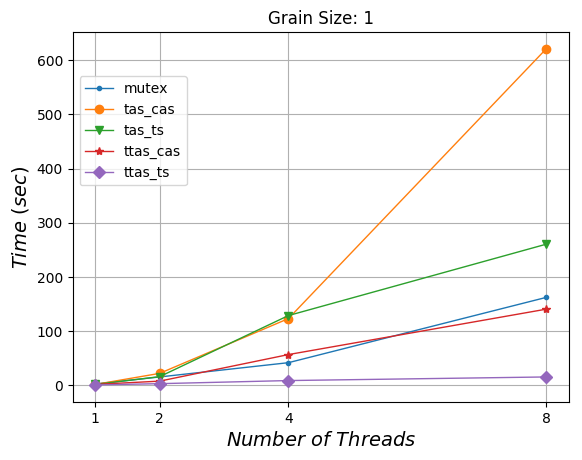
\includegraphics[width=0.7\textwidth]{./graphs/real/time/grain-1.png}
      \vspace{6mm}
   \end{center}
\end{minipage}

\begin{minipage}{\textwidth}
   \begin{center}
      \fbox{\textlatin{\textbf{\textit{Grain Size: 10}}}}\\
      \vspace{3mm}
      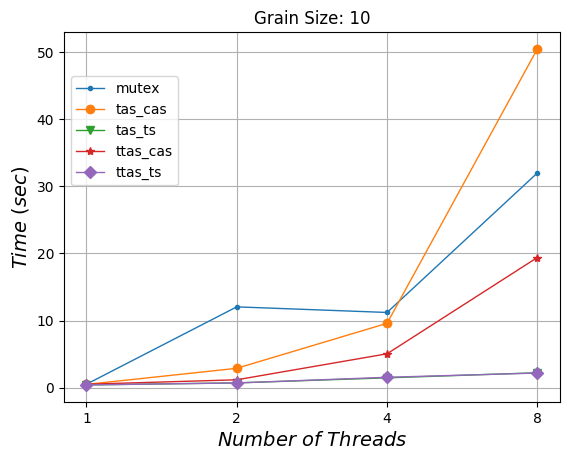
\includegraphics[width=0.7\textwidth]{./graphs/real/time/grain-10.png}
      \vspace{6mm}
   \end{center}
\end{minipage}

\begin{minipage}{\textwidth}
   \begin{center}
      \fbox{\textlatin{\textbf{\textit{Grain Size: 100}}}}\\
      \vspace{3mm}
      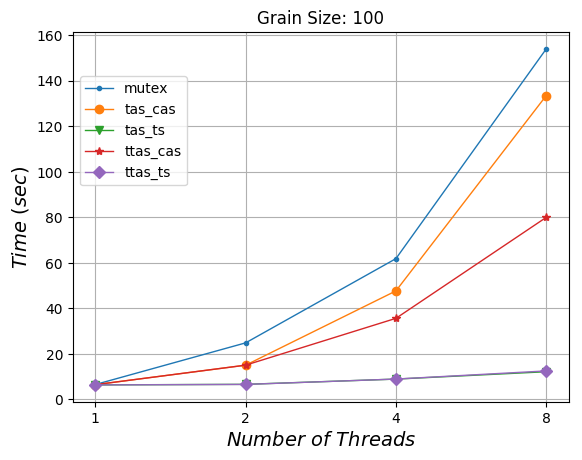
\includegraphics[width=0.7\textwidth]{./graphs/real/time/grain-100.png}
      \vspace{6mm}
   \end{center}
\end{minipage}

\paragraph{Συμπεράσματα - Σχόλια:}
Βλέπουμε πως κι εδώ η κλιμάκωση είναι σχεδόν γραμμική, όπως και τα αποτελέσματα
των προσομοιώσεων. Αυτό που είναι αξιοσημείωτο, είναι πως την βέλτιστη επίδοση
επιτυγχάνει το TTAS\_TS, με πολύ μεγάλη διαφορά στην μετρική του χρόνου σε
σύγκριση με τους υπόλοιπους μηχανισμούς. Μάλιστα, καθώς αυξάνεται το πλήθος των
πυρήνων σχεδόν ο χρόνος εκτέλεσης παραμένει σταθερός! 
Την επόμενη καλύτερη επίδοση σε όλα τα grain sizes παρουσιάζει το TTAS\_CAS,
δηλαδή ο ίδιος μηχανισμός υλοποιημένος με Compare and Swap atomic instructions. 

Είναι αξιοσημείωτο επίσης πως καθώς μεταβαίνουμε από τα 4 στα 8 νήματα, οι διαφορετικές
υλοποιήσεις του μηχανισμού TAS αποκλίνουν σημαντικά στην επίδοση, με την υλοποιήση του
TAS\_CAS να εμφανίζει χειρότερη επίδοση από τον TAS\_TS. Μάλιστα φαίνεται πως η επίδοση
του TAS\_CAS στις περισσότερες περιπτώσεις είναι παραπλήσια ή χειρότερη του MUTEX.
